
\begin{figure*}
	\centering
	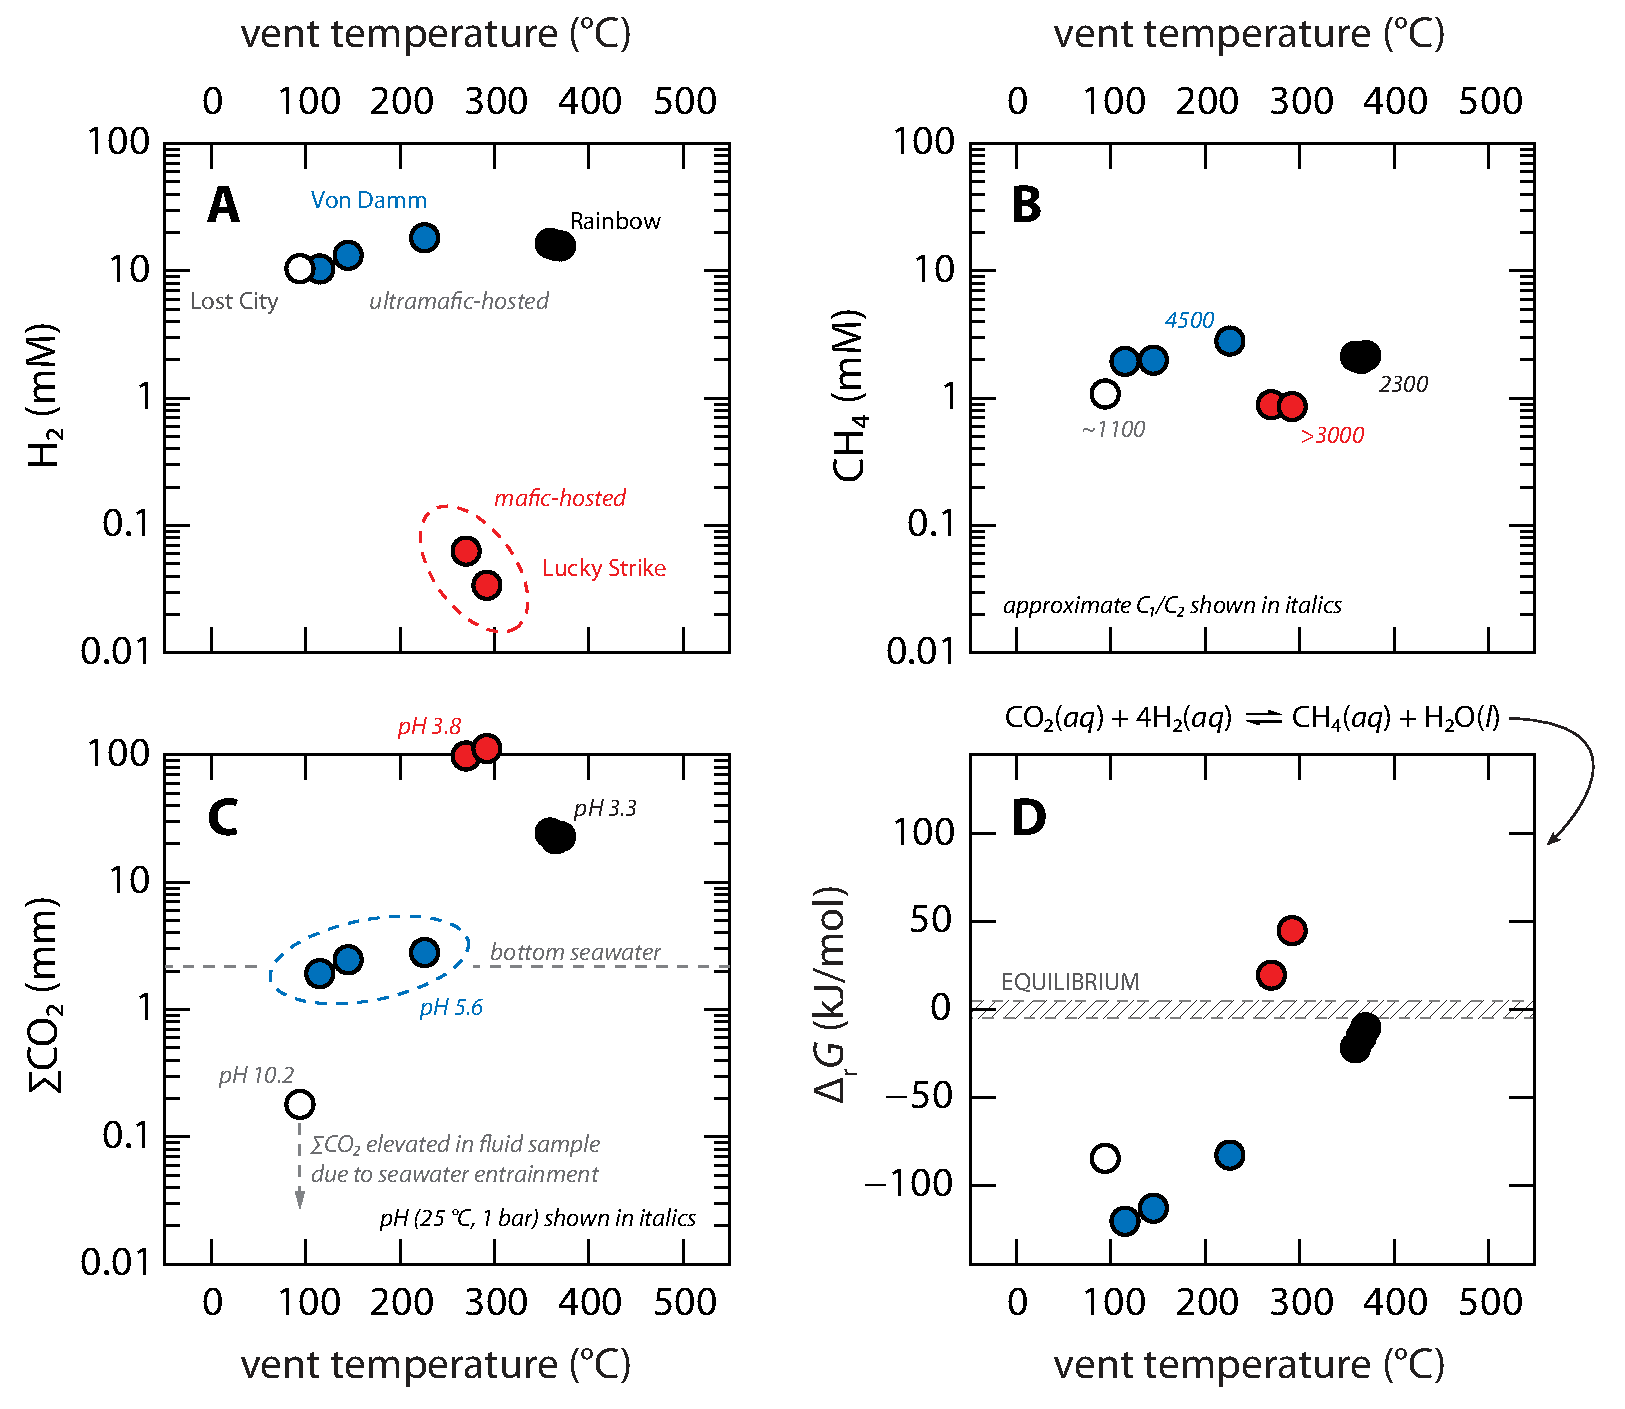
\includegraphics[width=0.95\linewidth]{figures/Fig3.3}
	\caption[Composition of vent fluids and energetics of methane synthesis in
		aqueous phase]{%
		Composition of vent fluids and energetics of methane synthesis in
		aqueous phase. Concentrations of (\textbf{A}) H\textsubscript{2},
		(\textbf{B}) CH\textsubscript{4}, and (\textbf{C}) $\big\sum\!$CO\textsubscript{2}
		are plotted against measured vent temperatures (data from \autoref{tab:3:2}). Also
		shown are molar ratios of methane to ethane
		(C\textsubscript{1}/C\textsubscript{2}, see \autoref{sec:3:results}) in (B), and pH
		values of endmember fluids in (C). (\textbf{D}) Gibbs energy of reaction
		for methane formation from CO\textsubscript{2} and H\textsubscript{2} in
		aqueous solution (\mrefs[]{Reaction}{eqn:3:2}), calculated at vent \emph{T} and \emph{P}
		conditions (Δ\textsubscript{r}\emph{G}, \autoref{tab:3:2}). Gray hatching
		represents thermodynamic equilibrium (taken as
		Δ\textsubscript{r}\emph{G} = 0 ± 5~kJ/mol). Methane formation in aqueous
		solution is thermodynamically favorable for points plotting below the
		hatched area. Symbol colors are the same as those in \mrefs[]{Figs.}{fig:3:1} and~\ref{fig:3:2}.
	}
	\label{fig:3:3}
\end{figure*}
